\chapter{Quantum digital signatures}
Goal of chapter: introduce our QDS protocol and prove its security in different contexts using several methods.

\MT{short introduction}

\section{Our QDS protocol}\label{sec:qds_protocol}

In the simplest instance we may consider a signature scheme involving only three parties: a sender, Alice ($A$), and recipients Bob ($B$) and Charlie ($C$). Alice wishes to send a classical message $m$ to $B$ and $C$, such that $B$ and $C$ can correctly determine whether $m$ was indeed sent by $A$. Furthermore the recipients should be able to check whether $m$ has been altered. The three-party setting is the smallest setting to fully distinguishes a digital signatures protocol from related protocols such as MACs \cite{Schneier2006}. Because more than two (potentially dishonest) players are present, this allows for attack strategies which are new from QKD and which make the QDS analysis distinct.

\subsection{QDS setup}

\begin{figure}[htp]
\centering

\includegraphics[width=0.8\linewidth, draft=false]{qds/qds_cartoon}
\caption{\label{fig:qds_cartoon} Setup of a $3$-party digital signatures scheme. Alice (A) wishes to securely sign her message $m$ such that Bob (B) and Charlie (C) both accept it as genuine.}
\end{figure}

Our signature scheme is displayed pictorially in Fig.~\ref{fig:qds_cartoon}. Alice (A) wishes to send a message $m$ to Bob (B) and Charlie (C) such that both Bob and Charlie accept it as genuine. To accomplish this she appends to $m$ a signature $\sigma_m$ which should be unique to the message and uniquely generated by Alice. In this way our digital signatures scheme is a quantum generalization of Lamport's protocol \MT{cite}. As we shall see later, any player in our protocol may be dishonest.

\subsection{Goals of a signature scheme}\label{sec:qds_goals}

A digital signature scheme must fulfill the following requirements

\begin{mylist}
\begin{enumerate}
\item\emph{Security against forgery}, Fig.~\ref{fig:attacks_forgery}. Neither a dishonest recipient ($B$ or $C$), nor an external fourth party (Eve, $E$), should be able to alter $m$ and have it accepted as genuine by an honest recipient. The signature scheme should ensure that $m$ is the message which Alice sent.

\item\emph{Genuine sender}, Fig.~\ref{fig:attacks_forgery}. Neither a dishonest recipient ($B$ or $C$), nor an external fourth party (Eve, $E$), should be able to impersonate $A$. A message which falsely claims to have originated with Alice should be rejected.

\item\emph{Security against repudiation}, Fig.~\ref{fig:attacks_repudiation}. A dishonest sender $A$ should not be able to cause disagreement between $B$, $C$ about the previous two requirements. After genuinely sending $m$ she should not later be able to deny it. If Bob accepts the message as genuine then so too should Charlie. 

\item \emph{Message transferability}, Fig.~\ref{fig:attacks_repudiation}. If $B$ accepts a message as genuine, then he should be sure that $C$ will also accept.

\item \emph{Robustness}, Fig.~\ref{fig:attacks_robustness}. The message $m$ should be accepted if all players behave honestly and there is no tampering by an eavesdropper.
\end{enumerate}
\caption{\label{list:qds_requirements} A secure QDS scheme should fulfill each of the above requirements. Requirement $1$ implies requirement $2$. In our $3$-party setting, requirements $3$ and $4$ are equivalent. We depict each type of attack which a QDS scheme must prevent in Fig.~\ref{fig:qds_attacks}.}
\end{mylist}

%Requirements $1$ and $2$ are fulfilled in our scheme by the same security process, and so we will focus on $1$ and simply note where $2$ arises.

If requirement $1$ holds then no dishonest player should be able to impersonate Alice, since in order to do so they will be required to generate $\sigma_m$ which at the start of the protocol is known only to her. The dishonest player's only hope then is to take Alice's place at the start of the protocol and perform a so-called ``man-in-the-middle'' attack. We do not investigate this possibilty further, though we note that without previous authenticated interaction between players even QKD is insecure for this attack \cite{Broadbent2015}.

For our scheme involving three parties, requirements $3$ and $4$ are equivalent. A QDS protocol involving $N$ recipients may distinguish between non-repudiation and transferability by defining a message $m^{\left(k\right)}$ as $k$-transferable if it may be successfully forwarded up to $k$ times. An honest participant should be able to determine the transferability level of $m$ \cite{Arrazola2016}. Non-repudiation then refers to Alice's ability to cause a message to be non-transferable. In what follows we treat these requirements as equivalent.

A digital signature scheme which rejects all messages trivially fulfills requirements $1-4$, and so in order to get a useful digital signature scheme we must also impose requirement $5$.

\begin{figure}[htp]
\centering
	\begin{subfigure}{\linewidth}
		\centering
		
\includegraphics[draft=false, width=\linewidth]{qds/qds_cartoon_forgery}
		\caption{\label{fig:attacks_forgery}}
	\end{subfigure}
	\begin{subfigure}{\linewidth}
		\centering
		
\includegraphics[draft=false, width=\linewidth]{qds/qds_cartoon_repudiation}
		\caption{\label{fig:attacks_repudiation}}
	\end{subfigure}
	\begin{subfigure}{\linewidth}
		\centering
		
\includegraphics[draft=false, width=\linewidth]{qds/qds_cartoon_honest_failure}
		\caption{\label{fig:attacks_robustness}}
	\end{subfigure}
\caption{\label{fig:qds_attacks} The multipartite setting permits many different methods for attack on the protocol depicted in Fig.~\ref{fig:qds_cartoon}. Gray boxes depict honest players while red boxes depict dishonest players. (a) Forging attack with dishonest Bob. Bob will change the message $m \rightarrow n$ with fake signature $sigma_n$. The attack succeeds if Charlie accepts. Alternatively, either Charlie or a fourth player, Eve, may attempt a forging attack. (b) Repudiation attack with dishonest Alice. Alice tries to convince Bob to accept the message and Charlie to reject it. (c) Honest failure. If all players behave honestly the protocol should succeed and both Bob and Charlie should accept the message.}
\end{figure}

\subsection{QDS protocol description}

We here present a continuous-variable (CV) QDS protocol based on the quadrature phase-shift keying (QPSK) alphabet of coherent states, Fig.~\ref{fig:qpsk}. %this will be defined earlier, I am sure
Our protocol allows us to take into account quantum distribution channels which will in general be insecure, and this scheme is the first in the CV setting to be secure against eavesdropping. %The physical setup of our scheme is depicted in Fig.~\ref{fig:qds_setup}, and the protocol is described fully in Ref.~\cite{Thornton2019}.

\begin{figure}[htp]
\centering
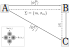
\includegraphics[draft=false, width=0.8\linewidth]{qds/qds_setup}
\caption{\label{fig:qds_setup} Setup of the QDS protocol considered in this chapter. Alice (A) wishes to securely sign a $1$~bit message $m$. Alice distributes quantum coherent states $\ket{\alpha \phi_j^{\left(B, C\right)}}$ along insecure quantum distribution channels (solid lines) during the Distribution stage. Bob and Charlie swap eliminated signature elements via their securely encrypted classical channel (dotted lines). During the Messaging stage Alice sends a message-signature $\Sigma$ pair along a classical broadcast channel (dot-dashed line). Inset: QPSK alphabet.}
\end{figure}

%\MT{Chat about the setup for our signatures scheme}

Our QDS scheme is split into two stages, Distribution and Messaging, which--by analogy with classical digital signatures--may occur with significant time delay. Quantum states are sent and measured during Distribution. During Messaging Alice will send her message and classical signature and recipients Bob and Charlie will try to determine its validity.\footnote{Note the intrinsic separation between the Distribution (quantum) and Messaging (classical) stages of the protocol. We will take further advantage of this separation between quantum and classical steps in Chapter~\ref{chapter:aqc}} Our protocol setup is outlined in Figs.~\ref{fig:qds_cartoon},~\ref{fig:qds_setup}. 
\par
\noindent We will now describe in detail the running of the protocol.


%\MT{mention somewhere why we consider just a $1$ bit message}

%\MT{I'll do everything for QPSK, but I should have a section where I generalize to NPSK}

\subsubsection{Distribution stage}

\paragraph{Step $1$.}
Alice wishes to send a signed $1$ bit message $m$ to Bob and Charlie. For each possible future $m$, and for each recipient, Alice creates the following classical strings
\begin{equation}
\Phi_m^{\left(B, C\right)} = \left\{ \phi_{j, m}^{\left(B, C\right)}\right\}_{j=1}^{L}
\end{equation}
where the $\phi_{j}$ are complex phases chosen from QPSK alphabet. The $\phi_j$ are assumed to be drawn uniformly at random, though we will relax this assumption in Chapter.~\ref{chapter:aqc}. The strings $\Phi_m^{\left(B, C\right)}$ may be interpreted as Alice's \emph{private key}. The signature length $L \in \mathbb{N}$ is chosen to ensure the desired level of security.

\paragraph{Step $2$.} Corresponding to each private key, Alice forms the following quantum states
\begin{equation}\label{eqn:QDS_publickey}
\rho\left[\Phi_m^{\left(B, C\right)}\right] := \otimes_{j=1}^L \; \rho\left[\phi_{j, m}^{\left(B, C\right)}\right]
\end{equation}
with
\begin{equation}
\rho\left[\phi_{j, m}^{\left(B, C\right)}\right] := \ket{\phi_{j, m}^{\left(B, C\right)}} \bra{\phi_{j, m}^{\left(B, C\right)}} \notag
\end{equation}
understood to be the coherent state from QPSK with phase corresponding to the relevant element of Alice's private key.

The states Eq.~\ref{eqn:QDS_publickey} may be interpreted simply as sequences of coherent states, and may be interpreted as Alice's \emph{public key}. An important difference between quantum and classical digital signatures is that here the public key may no longer be freely distributed, copied and stored. We also note that Alice no longer has a single public key. Indeed, her quantum public key differs both for each possible $m$ and for each recipient, which is a requirement for security against an eavesdropping forger. We shall discuss this at length in Sec.~\ref{sec:qds_security_forgery}.
\paragraph{Step $3$.}
Each recipient $B, C$ performs heterodyne detection Eq.~\ref{eqn:intro_heterodyne} on their received coherent states, and receives complex phase outcome $x_{\left(B, C\right)} \in \mathbb{C}$. Crucially, since measurement is performed immediately on receipt of the states no quantum memory is required. The remainder of the protocol is entirely classical.

\iffalse
%
% NOTE: I can stick this in my intro chapter.
%
each received $\rho\left[\phi_{j, m}^{\left(B, C\right)}\right]$ and receives complex phase outcome $x_{B,C}\in\mathbb{C}$. In other words, they perform the POVM
\begin{equation}
E\left[x\right] := \otimes_{j=1}^L E_j\left[x\right] \qq{with} E_j\left[x\right] := \frac{1}{\sqrt{\pi}} \ket{x}_j\bra{x}_j
\end{equation}
with $x \in \mathbb{C}$. 
\fi


At the end of the quantum stage of the protocol, recipients Bob and Charlie now possess classical strings, length $L$, containing their complex phase measurements on Alice's distributed states. They now form \emph{eliminated signatures}, Fig.~\ref{fig:elimsig}. For each outcome $x_j\in\mathbb{C}$, recipients record the phases $\phi_{j, m}^{\left(B, C\right)}$ which are \emph{least compatible} with $x_j$. For each entry $j$, this may be understood as computing the four conditional probabilities 
\begin{equation}
p\left(\alpha_j \given x_j\right) \qq{for each} \alpha_j \in \text{QPSK},
\end{equation}
and recording the $\alpha_j$ giving rise to the two smallest of these conditional probabilities.

Note that these recorded $\alpha_j$ will always be adjacent elements of QPSK. An example of this elimination procedure is displayed pictorially in Fig.~\ref{fig:elimsig}
%, and for clarity we display the mapping explicitly in Tab.~\ref{tab:elimsig}
. We denote Bob and Charlie's eliminated signatures at this stage as $X_m^{\left(B, C\right)}$. Each is of length $L$ and they will later be compared to Alice's private key in order to test the validity of the message.

\begin{figure}[htp]
\centering
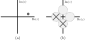
\includegraphics[draft=false, width=0.8\linewidth]{qds/elimsig}
\caption{\label{fig:elimsig} (a) Bob and Charlie each perform heterodyne outcome on their received coherent states, and measure complex outcome $x \in \mathbb{C}$. (b) They then record the two states from QPSK which are least likely to have been sent by Alice.}
\end{figure}

\paragraph{Step $4$. \emph{Symmetrization:}}
Bob and Charlie now swap a random $L/2$ elements of their $X_m^{\left(B, C\right)}$ over their encrypted classical channel. Signature elements which have been forwarded by a player will no longer be used by him in the protocol. We denote these resulting strings as $Y_m^{\left(B, C\right)}$. By using an encrypted classical channel the positions and values of swapped elements are kept secret from Alice, which will ensure that the information which Bob and Charlie each hold is symmetric from Alice's point of view \cite{Dunjko2014, Wallden2015}. 

In other words at the end of Step~$3$, having sent the state $\ket{\phi_{j, m}^B}\bra{\phi_{j, m}^B}$ to Bob, Alice knows that Bob holds the corresponding eliminated signature element $X_{j, m}^B$. Since Alice knows which state she sent to Bob, she may gain an advantage in trying to guess Bob's eliminated signature element. At the end of Step~$4$ however, Alice does not know whether it is Bob or Charlie who holds $X_{j, m}^B$. This uncertainty will prove crucial for preventing her from successfully repudiating (Requirement~$3$). 

Bob (and Charlie) now possesses an eliminated signature $\tilde{X}_m^{\left(B\right)}$ in two halves: one half ($Y_m^{\left(B\right)}$) containing those elements received directly from Alice, and one half ($Z_m^{\left(B\right)}$) containing elements received during this Symmetrization step from Charlie (Bob).

The key parameters for the Distribution stage are the signature length $L$, which directly measures the quantum resources required for the protocol, and the alphabet parameter $\alpha$ denoting the average photon number of the distributed coherent states. Channel parameters such as loss and thermal noise will be discussed later.\footnote{We will also later discuss an extension to the protocol which allows it to run with an $N$PSK alphabet of coherent states, where $N$ is an even integer.}

\subsubsection{Messaging stage}

Messaging may occur at any time after Distribution.

\paragraph{Step $5$.}
To sign $m$, Alice sends to Bob the classical information $\Sigma = \left(m, \sigma_m\right)$, consisting of the message which she would like to convey, and her private key $\sigma_m = \left(\Phi_m^B, \Phi_m^C\right)$ which acts as $m$'s signature. 


\paragraph{Step $6$.} Bob rearranges $\sigma_m \rightarrow \tilde{\sigma}_m^B := \left(\tilde{\Phi}_{Y, m}^B, \tilde{\Phi}_{Z, m}^B\right)$ by selecting elements from Alice's declaration which correspond to the two halves of his eliminated signature $\tilde{X}_m^{\left(B\right)}$. The original $\sigma_m$ has length $2 L$, while $\tilde{\sigma}_m^B$ has length $L$.

Bob compares relevant elements of $\tilde{\sigma}_m^B$ to his $\tilde{X}_m^{B}$, choosing which half of $\tilde{X}_m^B$ to compare to based on whether he kept or swapped the eliminated signature element. It is as this stage that Bob makes a decision about whether to accept $m$ as genuine. His decision will be based on Alice's declared $\tilde{\sigma}_m^B$, and the number of \emph{mismatches} between Alice's signature and his own eliminated signatures. A mismatch is defined in Sec.~\ref{sec:qds_mismatches} and in Fig.~\ref{fig:qds_mismatches}.


If Bob measures fewer than $s_B L/2$ mismatches on both of his eliminated signature halves then he accepts Alice's message as genuine, otherwise the protocol aborts. Bob's threshold mismatch rate $s_B$ determines how many mismatches he can observe before a signature fails his check. In general $s_B$ is a free parameter of the protocol and will be discussed further in Secs.~\ref{sec:qds_mismatches},~\ref{sec:qds_security_repudiation}.

%If Bob measures sufficiently few mismatches on both of his eliminated signature halves
%, i.e. if $\mathcal{M}\left(\tilde{\Phi}_{Y, m}^B, Y_m^B\right) < s_B L/2$ and $\mathcal{M}\left(\tilde{\Phi}_{Z,m}^B, Z_m^B\right) < s_B L/2$ 
%then he accepts Alice's declaration $m$ as genuine, otherwise the protocol aborts. %The threshold $0 \le s_B \le 1$ is related to the security of the protocol and will be discussed later.

\paragraph{Step $7$.} If Bob has accepted $m$, then he forwards $\Sigma$ to Charlie, who similarly checks for mismatches between Alice's signature and his eliminated signature. Charlie accepts the message if %$\mathcal{M}\left(\tilde{\Phi}_{Y, m}^C, Y_m^C\right) < s_C L/2$ and $\mathcal{M}\left(\tilde{\Phi}_{Z, m}^C, Z_m^C\right) < s_C L/2$, with security threshold $0 \le s_c \le 1$ to be discussed later. 
there are fewer than $s_C L/2$  mismatches between $\tilde{\sigma}_m^C$ and $\tilde{X}_m^{\left(C\right)}$. If Charlie also accepts $m$ then the protocol has succeeded, otherwise it aborts.  Charlie's threshold mismatch rate is $s_C$ and will be discussed further in Secs.~\ref{sec:qds_mismatches},~\ref{sec:qds_security_repudiation}.

The key parameters for the Messaging stage are $s_B, s_C$ which may be freely chosen by Bob and Charlie in order to optimize security.

%\clearpage
\subsection{Counting mismatches}\label{sec:qds_mismatches}

\begin{figure}[htp]
\centering
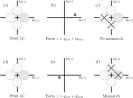
\includegraphics[draft=false, width=\linewidth]{qds/mismatch1}
\caption{\label{fig:qds_mismatches} A mismatch occurs when an honest party eliminates the state which Alice claims to have sent. (a, d) Alice sends coherent state $\ket{\alpha}$. (b, e) Bob (Charlie) heterodynes and measures $x \in \mathbb{C}$. Even when all players are honest there is some probability of measuring $\text{Re}\left(x\right) < 0$, Sec.~\ref{sec:qds_modelling_perr}. (c) Eliminated signature element consists of $\ket{- \alpha}, \ket{- i \alpha}$ so there is no mismatch. (f) Eliminated signature element consists of $\ket{\alpha}, \ket{i \alpha}$ and so there is a mismatch.}
\end{figure}


The key test of validity which our protocol employs is a check on the number of mismatches between Bob or Charlie's eliminated signatures $\tilde{X}^{\left(B, C\right)}_m$ and Alice's declaration $\sigma_m$. A mismatch occurs if the state which Alice claims to have sent has been eliminated, Fig.~\ref{fig:qds_mismatches}. 

To be concrete, a mismatch occurs at position $j$ if
\begin{equation}
\phi_{j, m}^B \in Y_{j, m}^B \qq{or} \phi_{j, m}^C \in Z_{j, m}^B, 
\end{equation}
and we let
\begin{equation}
\mathcal{M}\left(F, G\right)
\end{equation}
denote the probability of mismatch between an arbitrary eliminated signature $G$, and an arbitrary list of phases $F$. Both $F$ and $G$ should be of the same length.

%denote the probability of mismatch between arbitrary declared signature $F$ and arbitrary eliminated signature $G$.\MT{I think this should be more concrete}




\section{Security against repudiation}\label{sec:qds_security_repudiation}
\iffalse
In other words at the end of Step~$3$, having sent the state $\ket{\phi_{j, m}^B}\bra{\phi_{j, m}^B}$ to Bob, Alice knows that Bob holds the corresponding eliminated signature element $X_{j, m}^B$. Since Alice knows which state she sent to Bob, she may be able to guess Bob's eliminated signature element with some probability. 

 At the end of Step~$4$ however, Alice does not know whether it is Bob or Charlie who holds $X_{j, m}^B$. This uncertainty will prove crucial for preventing her from successfully repudiating (Requirement~$3$). Bob (and Charlie) now possesses an eliminated signature $\tilde{X}_m^{\left(B\right)}$ in two halves: one half ($Y_m^{\left(B\right)}$) containing those elements received directly from Alice, and one half ($Z_m^{\left(B\right)}$)containing elements received during this Symmetrization step from Charlie.
 \fi


We now turn to consider the security of the QDS protocol discussed in Sec.~\ref{sec:qds_protocol}. %Recall that of the five requirements for a digital signatures protocol, requirements $3$ and $4$ are equivalent in a $3$~party setting. 
In what follows we will prove that our protocol is:
\begin{enumerate}
\item Sec.~\ref{sec:qds_security_repudiation}: secure against a repudiation attack (List~\ref{list:qds_requirements}~requirement $3$, Fig.~\ref{fig:attacks_repudiation}), 
\item Sec.~\ref{sec:qds_security_robustness}: robust (List~\ref{list:qds_requirements} ~requirement $5$, Fig.~\ref{fig:attacks_robustness}),
\item Sec.~\ref{sec:qds_security_forgery} secure against a forgery attack (List~\ref{list:qds_requirements}~requirement $1$, Fig.~\ref{fig:attacks_forgery})
\end{enumerate}

Our proof will proceed by demonstrating that an attempted repudiation or forgery will induce a large mismatch rate, while a small mismatch rate is obtained when no attack is attempted. Thus, by appropriate choice of security parameters $s_B, s_C$ and signature length $L$, the probability of a \emph{successful} attack of any type may be made arbitrarily small. Proof security against repudiation follows along similar lines to Refs.~\cite{Dunjko2014, Wallden2015, Donaldson2016, Croal2016, Thornton2019}.

We assume that in our $3$~party setting at most \emph{one} of the players $A, B, C$ may behave dishonestly. For simplicity of notation we give a dishonest player the power to eavesdrop on the distribution of quantum states, and so the label $E$ is not required as an internal eavesdropper is at least as powerful as an external Eve. If two or more players are dishonest then we assume that they will collaborate, which allows them to trivially break the protocol and so this scenario is not discussed. We note that a collaboration of multiple dishonest players must be considered for an $n$~party QDS protocol, as discussed in Ref.~\cite{Arrazola2016}.

To succeed in a repudiation attack, a dishonest Alice aims to convince Bob that message $m$ is genuine, while Charlie that $m$ is fake, Fig.~\ref{fig:attacks_repudiation}. Security against repudiation is guaranteed by the Symmetrization procedure (Step $4$ of the protocol) which ensures that Alice does not know which recipient holds the eliminated signature element corresponding to a particular state which she sent. 

At the end of Step~$3$, having sent the state $\ket{\phi_{j, m}^B}\bra{\phi_{j, m}^B}$ to Bob, Alice knows that Bob holds the corresponding eliminated signature element $X_{j, m}^B$, and she may be able to guess it with high probability. In any case, knowing which recipient holds the $X_{j, m}^{\left(B, C\right)}$ gives Alice power to repudiate, even if she does not know what the individiual eliminated signature elements are\footnote{Alice could, for example, perform an optimal strategy in order to guess the $X_{j, m}^{\left(B, C\right)}$. Then she may declare $\sigma_m$ which uses her guesses on Bob's elements to reduce her mismatch rate with respect to Bob, while declaring the opposite of her guesses on Charlie's elements to increase her mismatch rate with respect to Charlie.}

At the end of Step~$4$ however, Alice does not know whether it is Bob or Charlie who holds an element $X_{j, m}^B$. This uncertainty will prove crucial for preventing her from successfully repudiating. Recall that Bob  (Charlie) possesses an eliminated signature $\tilde{X}_m^{\left(B\right)}$ in two halves: one half ($Y_m^{\left(B\right)}$) containing those elements received directly from Alice, and one half ($Z_m^{\left(B\right)}$) containing elements received during this Symmetrization step from Charlie (Bob).

We assume that Alice is completely free to manipulate her declared $\sigma_m = \left(\Phi_m^B, \Phi_m^C\right)$. We also assume that she may freely manipulate the number of mismatches %$\mathcal{M}\left(\Phi_m^{B, C}, X_m^{\left(B, C\right)}\right)$ 
between her declared signature and the eliminated signatures $X_m^{\left(B, C\right)}$ which Bob or Charlie held before Symmetrization. We denote these mismatch rates as $p_B$ and $p_C$, respectively, and Alice may even choose them to be zero

\begin{align}
p_B &= \mathcal{M}\left(\Phi_m^B, X_m^B\right) \notag \\
p_C &= \mathcal{M}\left(\Phi_m^C, X_m^C\right).
\end{align}

%After Symmetrization, Bob and Charlie each possess an eliminated signature in two halves, each of length $L/2$, consisting either of elements which they received directly from Alice, or of elements which they received during this step. 

Alice succeeds in her repudiation attack if Bob accepts both of his halves as genuine, while Charlie rejects at least one of his halves as fake. Let $E_A, E_B$ denote the events that Bob accepts on the first or second half of his eliminated signature, respectively. Let $E_C, E_C$ denote the events that Charlie rejects on the first or second half of his eliminated signature, respectively. Then a successful repudiation attack occurs when

\begin{equation}
\left(E_A \qq{and} E_B \right) \qq{and} \left( E_C \qq{or} E_D\right) \notag
\end{equation}
where the events are defined as
\begin{align}\label{eqn:repudiation_events}
&E_A \qq{when} \mathcal{M}\left(\tilde{\Phi}_{Y, m}^B, Y_m^B\right) < s_B L/2  \notag \\
%
&E_B \qq{when} \mathcal{M}\left(\tilde{\Phi}_{Z, m}^B, Z_m ^B\right) < s_B L/2 \notag \\
%
&E_C \qq{when} \mathcal{M}\left(\tilde{\Phi}_{Y, m}^C, Y_m^C\right) \ge s_C L/2 \notag \\
%
&E_D \qq{when} \mathcal{M}\left(\tilde{\Phi}_{Z, m}^C, Z_m^C\right) \ge s_C L/2 
\end{align}
where $\tilde{\Phi}$ denotes the rearranged form of Alice's declared phases $\Phi$ in order to compare corresponding elements, symbol $Y$ denotes that an element was received directly from Alice and symbol $Z$ denotes that it was received during Symmetrization. Function $\mathcal{M}$ measures the mismatch probability between two strings, and is defined above in Sec.~\ref{sec:qds_mismatches}.

Thus, the probability $\varepsilon_{\text{repudiation}}$ of a successful repudiation attack is given by

\begin{equation}
\varepsilon_{\text{repudiation}} = \text{P}\left[\left(E_A \cap E_B\right) \cap \left(E_C \cup E_D\right)\right].
\end{equation}
To proceed, we require the following two probability inequalities for arbitrary events $x, y$

\begin{align}
\label{eqn:prob_inequality_1}
\text{P}\left(x \cap y\right) &\le \text{min}\left\{\text{P}\left(x\right), \text{P}\left(y\right)\right\} \\
\label{eqn:prob_inequality_2}
\text{P}\left(x \cup y\right) &\le \text{P}\left(x\right) + \text{P}\left(y\right)
\end{align}
\noindent We may now use the probability inequality Eq.~\ref{eqn:prob_inequality_1} and observe that 

\begin{equation}
\varepsilon_{\text{repudation}} \le \text{min}\left\{\text{P}\left(E_A \cap E_B\right), \text{P}\left(E_C \cup E_D\right)\right\}. \notag
\end{equation}

\noindent Again using Eqs.~\ref{eqn:prob_inequality_1},~\ref{eqn:prob_inequality_2}, we arrive at

\begin{equation}\label{eqn:rep_prob_working}
\varepsilon_{\text{repudiation}} \le \text{min}\left\{
\text{min}\left\{\text{P}\left(E_A\right), \text{P}\left(E_B\right) \right\}, \text{P}\left(E_C\right) + \text{P}\left(E_D\right)\right\}
\end{equation}
which provides an upper bound for the probability of successful repudiation attack in terms of the individual probabilities for distinct events. We now wish to demonstrate that the probability for each event may be made arbitrarily small by suitable choice of $L$, and thus that $\varepsilon_{\text{repudiation}}$ may also be made arbitrarily small.


We rely on Hoeffding's inequalities Eqs.~\ref{eqn:hoeffding1},~\ref{eqn:hoeffding2} which we use to bound each probability appearing in Eq.~\ref{eqn:rep_prob_working}. Let $\mathcal{F}$ be a string of declared phases, and $\mathcal{G}$ be an eliminated signature. Strings $\mathcal{F}$ and $\mathcal{G}$ each have length $n$. We define a string $\mathcal{E}$ such that

\begin{equation*}\label{eqn:error}
\mathcal{E}_j = 
\begin{cases}
1 & \text{if $\mathcal{F}_j$ is eliminated in $\mathcal{G}_j$} \\
0 & \text{otherwise}
\end{cases}
\end{equation*}
which measures whether a mismatch has occurred between the $j^\text{th}$ elements of $\mathcal{F}$ and $\mathcal{G}$, Fig.~\ref{fig:qds_mismatches} Sec.~\ref{sec:qds_mismatches}.


The mismatch rate $\mathcal{M}\left(\mathcal{F}, \mathcal{G}\right)$ is equivalent to the empirical mean $\bar{\mathcal{E}}$, while its expectation $\mathbb{E}\left(\bar{\mathcal{E}}\right)$ is equal to the arithmetic mean
\begin{equation}
\mathbb{E}\left(\bar{\mathcal{E}}\right) = \frac{1}{n} \sum_{j=1}^n \mathcal{E}_j. \notag
\end{equation}

We wish to bound the probability that there are fewer than $s$ observed mismatches
\begin{equation}
\text{P}\left(\mathcal{M}\left(\mathcal{F}, \mathcal{G}\right) \le s\right) = \text{P}\left( \mathbb{E}\left(\bar{\mathcal{E}}\right) - \bar{\mathcal{E}} \ge \mathbb{E}\left(\bar{\mathcal{E}}\right) - s\right).
\end{equation}
Thus we have

\begin{equation}\label{eqn:qds_hoeffding1}
\text{P}\left(\mathcal{M}\left(\mathcal{F}, \mathcal{G}\right) \le s \right) \le \text{exp}\left(- 2 \left[\mathbb{E}\left(\bar{\mathcal{E}}\right) - s\right]^2 n \right)
\end{equation}
where the inequality follows from Hoeffding inequality Eq.~\ref{eqn:hoeffding1} provided that $\mathbb{E}\left(\bar{\mathcal{E}}\right) - s \ge 0$. This Eq.~\ref{eqn:qds_hoeffding1} provides an upper bound for the probability that there are fewer than $s$ mismatches observed when the average probability for mismatch is $\mathbb{E}\left(\bar{\mathcal{E}}\right)$

Similarly, we derive
\begin{equation}\label{eqn:qds_hoeffding2}
\text{P}\left(s \le \bar{\mathcal{E}}\right) \le \text{exp}\left( - 2 \left[s - \mathbb{E}\left(\bar{\mathcal{E}}\right)\right]^2 n\right)
\end{equation}
by applying Eq.~\ref{eqn:hoeffding2} provided that $s - \mathbb{E}\left(\bar{\mathcal{E}}\right) \ge 0$. This Eq.~\ref{eqn:qds_hoeffding2} provides an upper bound for the probability that there are more than $s$ mismatches observed when the average probability for mismatch is $\mathbb{E}\left(\bar{\mathcal{E}}\right)$. 


Using Eqs.~\ref{eqn:qds_hoeffding1},~\ref{eqn:qds_hoeffding2} we may now bound the probabilities for events Eq.~\ref{eqn:repudiation_events}

\begin{align}\label{eqn:qds_repudiation_events_probs}
\text{P}\left(E_A\right) \le \text{exp}\left( -\left[p_B - s_B\right]^2 L \right) \qq{provided that} p_B > s_B \notag \\
\text{P}\left(E_B\right) \le \text{exp}\left( -\left[p_C - s_B\right]^2 L \right) \qq{provided that} p_C > s_B \notag \\
\text{P}\left(E_C\right) \le \text{exp}\left( -\left[s_C - p_C\right]^2 L \right) \qq{provided that} p_C < s_C \notag \\
\text{P}\left(E_D\right) \le \text{exp}\left( -\left[s_C - p_B\right]^2 L \right) \qq{provided that} p_B < s_C
\end{align}

\noindent where in the first two inequalities we have applied Eq.~\ref{eqn:qds_hoeffding1} and in the second two inequalities we have applied Eq.~\ref{eqn:qds_hoeffding2}. Alice has the power to choose any $0 \le p_B, p_C \le 1$. We will consider some cases:

Assume that $p_B \ge s_B$. Then by the first inequality of Eq.~\ref{eqn:qds_repudiation_events_probs} the probability Eq.~\ref{eqn:rep_prob_working} must decay exponentially %must it? Could we decay faster? 
and so we are secure against repudiation. An analogous argument holds for the choice $p_C \ge s_B$ using the second inequality of Eq.~\ref{eqn:qds_repudiation_events_probs}.

Assume instead that $p_B < s_B$ and $p_C < s_B$. It follows that if we choose $s_B \le s_C$, then we force $p_B < s_C$ and $p_C < s_C$, and so Eq.~\ref{eqn:rep_prob_working} decays exponentially via the third and fourth inequalities of Eq.~\ref{eqn:qds_repudiation_events_probs}. Intuitively, we have demonstrated that even though Alice has full control over $p_B, p_C$ she cannot engineer a situation in which Bob measures fewer than $s_B$ mismatches while Charlie measures more than $s_C$. This relies on the choice $s_B \le s_C$, which ensures that $\varepsilon_{\text{repudiation}}$ decays exponentially in $L$.


Let us simplify Eq.~\ref{eqn:rep_prob_working}. Clearly, increasing $p_B$ or $p_C$ will cause both of the exponentials in the first term to decrease. Because of the inner minimum, we will only care about $\text{max}\left\{p_B, p_C\right\}$, and so we define $p := \text{max}\left\{p_B, p_C\right\}$ and write

\begin{equation}
\text{min}\left\{\text{exp}\left(- \left[p_B - s_B\right]^2L\right), \; \text{exp}\left(- \left[p_C - s_B\right]^2L\right)\right\} = \text{exp}\left(-\left[p - s_B\right]^2L\right). \notag
\end{equation}
In the case $p_B, p_C \le s_C$ we may increase the second term of Eq.~\ref{eqn:rep_prob_working} 

\begin{equation}
\text{exp}\left(- \left[s_C - p_C\right]^2 L \right) + \text{exp}\left(- \left[s_C - p_B\right]^2 L \right) \le 2 \exp\left( - \left[s_C - p\right]^2 L\right)
\end{equation}
and so

\begin{equation}
\varepsilon_{\text{repudiation}} \le \text{min}\left\{ 2 \text{exp}\left( - \left[p - s_B\right]^2 L \right), 2 \text{exp}\left( - \left[s_C - p\right]^2 L \right) \right\}.
\end{equation}
Since the minimum over two distinct Gaussians is maximized when the Gaussians have equal arguments, the probability $\varepsilon_{\text{repudiation}}$ is maximized when 
\begin{equation}
p = \frac{s_B + s_C}{2}.
\end{equation}

\noindent Finally, we reach
\begin{equation}\label{eqn:erep}
\varepsilon_{\text{repudiation}} \le 2 \text{exp}\left( - \frac{\left[s_C - s_B\right]^2}{4} L\right)
\end{equation}
as our useful bound for the probability that Alice succeeds in her repudiation attack. Since Eq.~\ref{eqn:erep} is exponentially decaying the probability that she succeeds may be made arbitrarily small by choice of $L$. We are therefore secure against repudiation attack.




\section{Robustness}\label{sec:qds_security_robustness}
The QDS protocol must be robust (List~\ref{list:qds_requirements} requirement~$5$, Fig.~\ref{fig:attacks_robustness}) and allow the message $m$ to be accepted provided that all parties behave honestly and there is no attack present. This is a requirement for \emph{useful} QDS, since a protocol which aborts for every message will certainly abort in the presence of an attack and thus is trivially secure. In this Section we will find an upper bound to the probability that the protocol fails even when everyone behaves honestly.

The protocol fails in the absence of attack if either Bob or Charlie rejects a message which Alice did in fact send, i.e. if Bob or Charlie detect too many mismatches on Alice's declaration $\sigma_m$. Since in Sec.~\ref{sec:qds_security_repudiation} we derived that $s_B \le s_C$, it will always be more likely that Bob rejects than Charlie. We will seek to bound the probability that Bob measures more than $s_B L/2$ mismatches on either of his signature halves. This will also provide an upper bound for the probability that Charlie rejects with no attack.

We define an \emph{honest mismatch} to have occured if there is a mismatch between Alice's declaration and either of Bob's (or Charlie's) eliminated signature halves in an honest scenario. Let $\perr$ be the probability of honest mismatch. Because of the non-orthogonality of coherent states even in an ideal setting we have $\perr > 0$. This is in contrast to protocols such as Refs.~\cite{Donaldson2016, Collins2014} which could attain an ideal $\perr = 0$. We model $\perr$ in the next Section~\ref{sec:qds_modelling_perr} and there demonstrate that it is nonzero.

Using probability inequality Eq.~\ref{eqn:prob_inequality_2}, the probability that Bob rejects either of his halves is given by

\begin{equation}
\varepsilon_{\text{Bob rejects}} \le 2 \text{P}\left(E_A\right)
\end{equation}
where $E_A$ is the event that Bob measures more than $s_B L/2$ mismatches on either of his halves. We have implicitly assumed that $\perr$ is identical for states originally sent to Bob and those originally sent to Charlie, but this is easy to relax if desired.

Using Hoeffding inequality Eq.~\ref{eqn:qds_hoeffding2} in an identical manner to the derivation of Eq.~\ref{eqn:qds_repudiation_events_probs}, Sec.~\ref{sec:qds_security_repudiation}, we see that
\begin{equation}\label{eqn:ehonabort}
\varepsilon_{\text{honest abort}} = \varepsilon_{\text{Bob rejects}} \le 2 \exp\left( - \left[s_B -\perr\right]^2 L\right)
\end{equation}
provided that $s_B - \perr \ge 0$. Equation~\ref{eqn:ehonabort} is our useful bound for the probability that the protocol fails the robustness requirement. Since it is exponentially decaying the probability that this happens can be made arbitrarily small, and so our protocol is robust.

\subsection{Modelling $p_{\text{err}}$}\label{sec:qds_modelling_perr}

The probability $\perr$ corresponds to the probability that a heterodyne measurement outcome $z$ has $\text{Re}\left(z\right) < 0$ when Alice distributed the coherent state $\ket{\alpha}$, Fig.~\ref{fig:perr}. In the absence of thermal noise the channel simply acts as a beamsplitter with vacuum at the fourth port, and so

\begin{equation}
\ket{\alpha}_A \rightarrow \ket*{\sqrt{T}\alpha}_{\left(B, C\right)}
\end{equation}


\noindent when the channel has transmittivity $T$. A heterodyne measurement on the output state gives outcome $z \in \mathbb{C}$ with probability
\begin{align}
\text{P}\left(z\right) = \langle z | \sqrt{T}\alpha\rangle\langle\sqrt{T}\alpha|z\rangle = \left|\langle z | \sqrt{T} \alpha \rangle \right|^2& \notag \\
= \frac{1}{\pi}\text{exp}\left( - \left| z - \sqrt{T}\alpha \right|^2 \right)&
\end{align}
where ket vector $|z\rangle$ denotes the coherent state centred on $z$. Then,

\begin{align}
\perr &= \text{P}\left(\text{Re}\left(z\right)<0\right) = \int\limits_{\text{Re}\left(z\right)<0}\Diff2 z \, \text{P}\left(z\right) \notag \\
&= \int\limits_{-\infty}^{\infty} \mathrm{d} y \, \text{exp}\left(-y^2\right) \int\limits_{-\infty}^{0} \mathrm{d} x \, \text{exp}\left(-\left[x - \sqrt{\frac{T}{2}}\alpha_x\right]^2\right)
\end{align}
where the factor $1/\sqrt{2}$ arises from Eq.~\MT{X} %the one relating quadratures and complex phase
and where $x = \text{Re}\left(z\right), y = \text{Im}\left(z\right)$ and $\alpha_x = \text{Re}\left(\alpha\right)$. 

Integrating, we arrive at

\begin{equation}\label{eqn:perr}
\perr = \frac{1}{2}\text{erfc}\left(\sqrt{\frac{T}{2}}\alpha\right)
\end{equation}

\noindent which models the probability of honest mismatch over a lossy channel with transmittivity $T$. Probability $\perr$ is motivated in Fig.~\ref{fig:perr} which elucidates the above discussion, and explains why $\perr \ne 0$. An equivalent analysis when the channel containst thermal noise is discussed in Sec.~\MT{X}

\begin{figure}[htp]
\centering
\includegraphics[draft=false, width=0.5\linewidth]{qds/perrnonzero}
\caption{\label{fig:perr} Histogram of possible heterodyne outcomes. A coherent state $\ket{\alpha}$ with $\alpha>0$ has nonzero probability to give measurement outcome $z \in \mathbb{C}$ with $x = \text{Re}\left(z\right) < 0$. In other words, $\perr > 0$ always, and $\perr \rightarrow 0$ only as $\alpha \rightarrow \infty$. The blue region corresponds to measurement outcomes which will not give a mismatch, while the pink region corresponds to measurement outcomes which will yield a mismatch. $x = \text{Re}\left(z\right), y = \text{Im}\left(z\right)$. This histogram is equivalent to the Hussimi $Q$ function \cite{Leonhardt2010} of the received coherent state and is thus also Gaussian.}
\end{figure}


\section{Security against forgery}\label{sec:qds_security_forgery}
We now turn to consider security against forgery, List.~\ref{list:qds_requirements}~requirement $1$, Fig.~\ref{fig:attacks_forgery}. In a forging attack, a dishonest player (or a fourth party, Eve) will declare some fake $m^\prime$ with the aim that it should be accepted by honest players as being genuine and originating with Alice. % In this attack we consider two possibilities, either that an honest Alice's $\Sigma$ has been intercepted and altered (interferance in Step $5$); or that honest Alice has completed distribution of quantum states, Step $3$, but has not yet sent $\Sigma$. As should be clear from the following discussion 
We will not consider the possibility that a dishonest player is impersonating Alice from the beginning of the protocol (see Sec.~\ref{sec:qds_goals} for brief discussion). The fake message $m^\prime$ will have an appended signature $\tau_{m^\prime}$ consisting of declared coherent state phases. Message $m^\prime$ will be accepted if $\tau_{m^\prime}$ has sufficiently few mismatches with respect to an honest player's eliminated signature. 

%Since Bob already knows $L/2$ of Charlie's elements, precisely those $Z_m^C$ which originated with Bob,

Since Bob and Charlie already know $L/2$ of each other's eliminated signature elements--those which were forwarded during the Symmetrization step of the protocol--a dishonest player who is internal to the signature scheme will have an advantage over an external Eve. Additionally, since $s_B < s_C$, Charlie is more likely than Bob to accept a forged message $m^\prime$ and fake signature $\sigma_{m^\prime}$, and so the most dangerous forger will be a dishonest Bob. We thus proceed with the mantra ``Bob is Eve'' and take Bob as our dishonest, forging party. Since the worst-case scenario is a forging Bob, our following analysis will implicitly also guard against the possiblity that Charlie or Eve are the forger.

Since Bob already knows the $L/2$ elements $Z_{m}^C$ which Charlie received from Bob during Symmetrization, Step $4$, Bob is able to cause arbitrarily few mismatches on that half of Charlie's signature. Bob's goal then is to declare a string $\tilde{\Phi}^C_{Y, m^\prime}$, length $L/2$ such that 
\begin{equation}\label{eqn:forging_condition}
\mathcal{M}\left(\tilde{\Phi}^C_{Y, m^\prime}, Y_{m^\prime}^C\right) \le s_C \frac{L}{2}
\end{equation}
which will be accepted by Charlie.

Bob's only strategy to gain information about the $Y_{m^\prime}^C$ is to eavesdrop on the distribution of states from Alice to Charlie during Steps~$2$ and $3$ of the protocol, and Bob's eavesdropping strategies will be fully considered in Sec.~\ref{sec:qds_attack_analysis}, below.

Defining $\text{p}_e$ as the probability that Bob will induce a mismatch on an individual given signature element, the probability $\varepsilon_{\text{forgery}}$ that Bob succeeds in his forging attack is
\begin{equation}\label{eqn:eforg}
\varepsilon_{\text{forgery}} \le 2 \text{exp}\left( - \left[\text{p}_e - s_C\right]^2 L\right), 
\end{equation}
provided that $\pe - s_C \ge 0$. Equation~\ref{eqn:eforg} is derived using Eq.~\ref{eqn:qds_hoeffding1} similarly to Eqs.~\ref{eqn:erep},~\ref{eqn:ehonabort} in Secs.~\ref{sec:qds_security_robustness},~\ref{sec:qds_security_robustness} by calculating the probability that Charlie accepts a message with more than $\pe$ mismatches.

Charlie's threshold $s_C$ may be freely chosen, and by combining it with conditions required for derivation of Eqs.~\ref{eqn:erep},~\ref{eqn:ehonabort} we deduce the requirement
\begin{equation}\label{eqn:qds_security_condition}
\perr \le s_B \le s_C \le \pe 
\end{equation}
where threshold parameters $s_B, s_C$ may be freely chosen to optimize security. 

Equation~\ref{eqn:qds_security_condition} encodes the intuitive condition that the QDS protocol is secure provided that $\pe \ge \perr$; or, in other words, that a dishonest forger will cause more mismatches than an honest player. The protocol security analysis thus relies on finding alphabet parameters and channels for which a forger is guaranteed to make more errors than the honest error rate $\perr$, and thus for which a forging attack will be detectable. In Sec.~\ref{sec:qds_bounding_pe} we demonstrate how $\pe$ relates to the quantum system held by Bob at the end of the protocol's Distribution stage, while in Sec.~\ref{sec:qds_attack_analysis} we analyse several types of eavesdropping attack which Bob may attempt, and we perform several explicit calculations of $\pe$ under different channel conditions.

%\MT{Make a statement comparing this $\pe \ge \perr$ condition to QKD, where an eavesdropper can hide an attack below channel noise.}

\section{Bounding $\pe$}\label{sec:qds_bounding_pe}
To complete the security analysis of our protocol, and in order to compute an upper bound for $\varepsilon_{\text{fail}}$, Eq.~\ref{eqn:efail}, we must find a lower for $\pe$, the rate at which a forging Bob will induce a mismatch with respect to Charlie's signature. Our protocol may be secured provided that $\pe > \perr$ and an honest Charlie outperforms dishonest Bob. The key contribution of this section will be a lower bound for $\pe$ which may be calculated once Bob's quantum system at the end of the Distribution stage of the protocol is known.

%, while fully taking into account the ambiguity in Bob's declaration.

%This ambiguity stems from the following. Because Charlie eliminates two states from $\mathcal{A}_4$, Fig.~\ref{fig:elimsig}, there are

%\begin{figure}[htp]
%\centering
%\includegraphics{ambiguity.png}
%\end{figure}

Bob will declare a string $\tilde{\Phi}_{Y, m^\prime}^C$, length $L/2$,  aimed to cause sufficiently few mismatches with respect to Charlie. For convenience we will abbreviate Bob's declared string as $\tilde{\Phi}_{\text{Bob}}$. %Our security analysis must fully take into account the ambiguity in Bob's declarations. This ambiguity stems from the following, and is illustrated in Fig.~\ref{fig:ambiguity}. 
The analysis differs from QKD analysis in that Bob's mismatch probability is \emph{not equivalent} to the probability that he misidentifies an element of Chalie's eliminated signature\footnote{And so a Helstrom-like approach \MT{define} will not work. We will pick up this idea further for comparison with our mismatch-based protocol in Sec.~\ref{sec:qds_helstromlike}.} Because Charlie eliminates two states from QPSK, Fig.~\ref{fig:elimsig}, there are remaining two states from the QPSK alphabet which Bob can declare without introducing a mismatch. Each of the remining states is shared with another possible eliminated signature element, and so it is possible that Bob misidentify Charlie's eliminated signature and yet still not introduce a mismatch.

This forces us to work directly in terms of mismatch probability $\pe$, which we do via our error variable $\mathcal{E}$, Eq.~\ref{eqn:error}, the $j^{\text{th}}$ element of which is $1$ if Bob induces a mismatch, and $0$ if there is no mismatch. We will continue to work in terms of the QPSK alphabet, though in Sec.~\ref{sec:qds_larger_alphabets} we will show how the proof may be generalized to an $N$PSK alphabet.

To proceed, recall that $Y_{m^\prime}^C$ is the half of Charlie's eliminated signature based on states he received directly from Alice. This is the half which Bob will attack. We define $Y_j$ to be its $j^{\text{th}}$ element, and write $Y_j = \left\{ y_1^j, y_2^j\right\}$ for $y_1^j, y_2^j$ phases in QPSK alphabet. The $y_{1,2}^j$ denote the states which Charlie has eliminated. Note that $y_{1,2}^j$ must be adjacent to each other in phase-space, that is, if $y_1^j = \alpha$ then $y_2^j$ must be either $i \alpha$ or $- i \alpha$. The string $\tilde{\Phi}_{\text{Bob}} = \left\{\phi_j\right\}_{j=1}^{L/2}$ is Bob's declaration, which is the result of an unspecified but optimal POVM and classical strategy.

A mismatch occurs when $\phi_j = y_1^j$ or $\phi_j = y_2^j$. Bob's average mismatch rate $\pe$ may be equivalently written in terms of $\mathcal{E}$
\begin{equation}
\pe = \text{P}\left(\mathcal{E}_j = 1\right). \notag
\end{equation}
Because $\mathcal{E}_j$ can take one of two values, the Shannon entropy $\text{H}\left(\mathcal{E}_j\right)$ is equivalent to the binary entropy $\text{h}\left(\pe\right)$, which is defined in Eq.~\ref{eqn:intro_binary_entropy}. %define this equation in introduction chapter.

Now, consider the conditional entropy
\begin{equation}
\text{H}\left(\mathcal{E}_j, y_1^j, y_2^j \given \phi_j\right)
\end{equation}
which is related to the uncertainty about whether a mismatch has occurred under Bob's declaration $\phi_j$. Using the chain rule for conditional entropies, Eq.~\ref{eqn:intro_chain_rule}, we may write
\begin{equation}\label{eqn:qds_pe_deriv_1}
\text{H}\left( \mathcal{E}_j, y_1^j, y_2^j \given \phi_j \right) = 
\text{H}\left( \mathcal{E}_j \given y_1^j, y_2^j, \phi_j\right) + 
\text{H}\left( y_1^j, y_2^j \given \phi_j\right).
\end{equation}
Since an element $\mathcal{E}_j$ is uniquely determined once $\phi_j, y_1^j, y_2^j$ are known, we may immediately deduce
\begin{equation}
\text{H}\left( \mathcal{E}_j \given y_1^j, y_2^j, \phi_j\right) = 0. \notag
\end{equation}

\noindent Using chain rule Eq.~\ref{eqn:intro_chain_rule} once again on the left hand side of Eq.~\ref{eqn:qds_pe_deriv_1}, but this time expanding over variable $y_1^j, y_2^j$,
\begin{align}\label{eqn:qds_pe_deriv_2}
\text{H}\left( \mathcal{E}_j, y_1^j, y_2^j \given \phi_j \right) &=
\text{H}\left(y_1^j, y_2^j \given \mathcal{E}_j, \phi_j\right) + \text{H}\left(\mathcal{E}_j \given \phi_j\right) \notag \\
&\le \text{H}\left(y_1^j, y_2^j \given \mathcal{E}_j, \phi_j\right) + \text{H}\left(\mathcal{E}_j\right) \notag \\
&= \text{H}\left(y_1^j, y_2^j \given \mathcal{E}_j, \phi_j\right) + \text{h}\left(\pe\right)
\end{align}
where the inequality follows because conditioning cannot increase entropy, Eq.~\ref{eqn:intro_conditioning_cannot_increase}.

Combining Eqs.~\ref{eqn:qds_pe_deriv_1} and \ref{eqn:qds_pe_deriv_2},

\begin{align}\label{eqn:qds_pe_deriv_3}
\text{H}\left(y_1^j, y_2^j \given \phi_j\right) &\le \text{H}\left(y_1^j, y_2^j \given \mathcal{E}_j, \phi_j\right) + \text{h}\left(\pe\right) \notag \\
&= \text{P}\left(\mathcal{E}_j=0\right) \text{H}\left(y_1^j, y_2^j \given \mathcal{E}_j=0, \phi_j\right) \notag \\
&+ \text{P}\left(\mathcal{E}_j=1\right) \text{H}\left(y_1^j, y_2^j \given \mathcal{E}_j=1, \phi_j\right) + \text{h}\left(\pe\right)
\end{align}
with
\begin{equation}
\text{P}\left(\mathcal{E}_j=0\right) = 1 - \pe \qq{and} \text{P}\left(\mathcal{E}_j=1\right) = \pe.
\end{equation}

\noindent Now, because there are two eliminated signature elements consistent with a given $\mathcal{E}_j=0$ and $\phi_j$, and since we are free to permute and relabel $y_1^j \leftrightarrow y_2^j$, we have four choices for the variable $y_1^j, y_2^j$ once $\mathcal{E}_j$ and $\phi_j$ are chosen\footnote{And eight choices \emph{a priori}.}. Thus,
\begin{equation}
\text{H}\left(y_1^j, y_2^j \given \mathcal{E}_j=0, \phi_j\right) \le \log_2 4 = 2.
\end{equation}

\noindent Additionally, since Charlie eliminates precisely half of $\mathcal{A}_4$ to form his eliminated signature, we see that
\begin{equation}
\text{H}\left(y_1^j, y_2^j \given \mathcal{E}_j=0, \phi_j\right) = \text{H}\left(y_1^j, y_2^j \given \mathcal{E}_j=1, \phi_j\right),
\end{equation}
and so Eq.~\ref{eqn:qds_pe_deriv_3} becomes
\begin{equation}\label{eqn:qds_pe_deriv_4}
\text{H}\left(y_1^j, y_2^j \given \phi_j\right) \le 2 + \text{h}\left(\pe\right).
\end{equation}

\noindent Let us expand the left hand side of Eq.~\ref{eqn:qds_pe_deriv_4} using the definition of mutual information, Eq.~\ref{eqn:intro_mutual_information}:
\begin{equation}\label{eqn:qds_pe_deriv_5}
\text{H}\left(y_1^j, y_2^j \given \phi_j\right) = \text{H}\left(y_1^j, y_2^j\right) - \text{I}\left(y_1^j, y_2^j : \phi_j\right).
\end{equation}

\noindent There are four possible eliminated signature elements, therefore eight possible choices for $y_1^j, y_2^j$ including relabeling $y_1^j \leftrightarrow y_2^j$, and so 
\begin{equation}
\text{H}\left(y_1^j, y_2^j\right) = \log_2 8 = 3.
\end{equation}

\noindent Additionally, we lower bound Eq.~\ref{eqn:qds_pe_deriv_5} by using the fact that the Holevo information maximizes the mutual information over all POVMs, Sec.~\ref{sec:Holevo}, and so
\begin{equation}\label{eqn:qds_pe_deriv_6}
\text{H}\left(y_1^j, y_2^j \given \phi_j \right) = 3 - \chi\left(y_1^j, y_2^j : \phi_j\right).
\end{equation}

\noindent Finally, combining Eqs.~\ref{eqn:qds_pe_deriv_4} and \ref{eqn:qds_pe_deriv_6} we arrive at
\begin{equation}\label{eqn:qds_hpe}
\text{h}\left(\pe\right) \ge 1 - \chi \left(y_1^j, y_2^j : \phi_j\right)
\end{equation}
which is one of the key results for this chapter, and a key result of Ref.~\cite{Thornton2019}. Because we have used the Holevo information, we automatically include dishonest Bob's optimal POVM and classical strategy. Thus, the bound Eq.~\ref{eqn:qds_hpe} is a useful one provided that we are able to calculate $\chi$. In the following sections we will consider some realistic cases where this is possible.

Since binary entropy $\text{h}\left(\pe\right)$ is monotonic for $\pe \le 1/2$, Fig.~\ref{fig:binary_entropy}, we conclude that a lower bound for $\text{h}\left(\pe\right)$ also gives us a lower bound for $\pe$. The inequality~\ref{eqn:qds_hpe} is solved for Bob's average mismatch rate $\pe$, which may then be combined with $\perr$ in order to calculate $\varepsilon_{\text{forgery}}$, Eq.~\ref{eqn:eforg}

%and provide security against collective attacks \MT{define} provided that Bob's Holevo information $\chi$ can be estimated.

\section{Attack analysis}\label{sec:qds_attack_analysis}
We will consider several different models of dishonest Bob's eavesdropping attack. Different models will affect both the parameter regimes over which our protocol can be made secure, and the cost of resources required for that security. We will demonstrate how Bob's Holevo information may be calculated in each model, which may then be used to calculate $\pe$, Eq.~\ref{eqn:qds_hpe}.

As in the QKD literature \cite{Lutkenhaus2004} we define the following three types of quantum attack, which are displayed in Fig.~\ref{fig:types_of_attack}.
\begin{itemize}
\item individual: Fig.~\ref{fig:types_of_attack_individual}
\item collective: Fig.~\ref{fig:types_of_attack_collective}
\item coherent: Fig.~\ref{fig:types_of_attack_coherent}
\end{itemize}
In an individual attack, Fig.~\ref{fig:types_of_attack_individual}, Bob interacts separately with each signal state distributed from Alice to Charlie, and performs separate measurements on each state. For a collective attack, Fig.~\ref{fig:types_of_attack_collective}, Bob again interacts with each signal state separately, but is permitted to perform a global measurement on his entire quantum system. This may include either introducing or exploiting classical correlations between signal states. Finally, in a coherent attack, Fig.~\ref{fig:types_of_attack_coherent}, Bob interacts with all signal states globally and (assumed) simultaneously, and he is permitted to perform a global measurement on his entire system. This attack affords him the full power of quantum mechanics and he can perform anything which is physically consistent, including introducing and exploiting quantum correlations between signal states.


\begin{figure}[htp]
\centering
	\begin{subfigure}{\linewidth}
		\centering
			\caption{\label{fig:types_of_attack_individual}}
		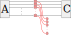
\includegraphics[width=0.4\linewidth, draft=false]{qds/individual_attacks}
	\end{subfigure}
	\begin{subfigure}{\linewidth}
		\centering
		\caption{\label{fig:types_of_attack_collective}}	
		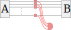
\includegraphics[width=0.4\linewidth, draft=false]{qds/collective_attacks}
	\end{subfigure}
	\begin{subfigure}{\linewidth}
		\centering
		\caption{\label{fig:types_of_attack_coherent}}	
		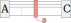
\includegraphics[width=0.4\linewidth, draft=false]{qds/coherent_attacks}
	\end{subfigure}
\caption{\label{fig:types_of_attack} Taxonomy of different eavesdropping attack strategies \cite{Lutkenhaus2004}. Gray arrows denote quantum signal states distributed from Alice to Charlie. Red items belong to Bob. (a) Individual attack. Bob inserts separate probes (red boxes) into state distribution and performs measurement on each system individually. (b) Collective attack. Bob inserts separate probes into state distribution and stores his states until the end of signal distribution. He may then perform a measurement on her entire system. (c) Coherent attack. Bob interacts with all signals at the same time and he can perform a measurement on a single probe. Attack (a) cannot introduce correlations between signals. Attack (b) may introduce classical correlations, and attack (c) may introduce any correlations between signals.}
\end{figure}

\MT{--------------------------------------}


In this section we will focus on individual and collective forging attacks. Full security against coherent quantum attacks in the CV QKD literature has only been proven for the simpler case of coherent states modulated with a Gaussian distribution \cite{Lodewyck2007, Leverrier2010c, Pirandola2008, Leverrier2015, Laudenbach2017, Furrer2012}, and a full security proof remains elusive for a discrete modulation of coherent states. There has been some recent success in applying convex optimization methods to the problem \cite{Ghorai2019, Lin2019}, but these proofs rely on an assumption about the Gaussianity of the discretely modulated alphabet \cite{Leverrier2009} which is only valid as $\alpha \rightarrow 0$. In keeping with recent trends in the QKD literature for the discrete modulation of coherent states without a Gaussian assumption \cite{Papanastasiou2018}, we will focus on bounding the attack strength of individual attack, and then assume the i.i.d. criterion \cite{Leverrier2017, Laudenbach2017}, to reach security against collective attack. 

%In the QKD literature it was demonstrated \MT{cite} that under \MT{conditions}, security against the collective attack may be proven in terms of security against individual attack. \MT{demonstrate (or motivate) that the same should be true here.}


In particular, we will study both the beamsplitter attack and the entangling cloner attack for our protocol \cite{Grosshans2002, Grosshans2003}. In both of these attacks the quantum distribution channel will be replaced, by Bob and hidden from Alice and Charlie, with a beamsplitter intended to mimic the effect of the channel on Charlie's measurement outcomes. In particular, Bob will either input into the channel the vacuum state, a thermal state Eq.~\ref{eqn:intro_thermal}, or one arm of his two-mode entangled state Eq.~\ref{eqn:intro_tmsv}.

\subsection{Beamsplitter attack}

\begin{figure}[htp]
\centering
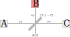
\includegraphics[draft=False,width=0.8\linewidth]{qds/BS0}
\caption{\label{fig:bs0_attack} Attack BS$0$. Bob replaces the channel with a beamsplitter in order to mimic channel loss. By inputting vacuum $\ket{0}$ into the beamsplitter Bob mimics channel loss while imposing zero excess noise.}
\end{figure}
In its canonical form, the beamsplitter attack, Fig.~\ref{fig:bs0_attack}, allows Bob to replace a lossy channel, transmittivity $T$ with a corresponding beamsplitter. Bob inputs vacuum $\ket{0}$ into the fourth port, and as such introduces no noise into the channel. Bob receives his quantum system $\rho_B$ from the reflected output port, and from $\rho_B$ he will attempt to gain information about Charlie's measurement outcomes. Crucially, to honest players Alice and Charlie this attack is indistinguishable from simply having a lossy transmission channel, and so in analysis all channel loss must be attributed to the action of the dishonest Bob. 

Since in the usual beamsplitter attack Bob inputs only vacuum into the beamsplitter's fourth port, this form of attack cannot model any channel excess noise $\xi$ and it should therefore be ignored in the analysis. However, a realistic channel will impose noise onto Charlie's measurement outcomes, and we describe some modifications to the beamsplitter attack in Secs.~\ref{sec:qds_bs1},~\ref{sec:qds_bs2}. 

%However, in order to include excess noise in our analysis, we will examine two modifications to the standard beamsplitter attack. Each modification to the standard beamsplitter attack will be discussed in turn, and then we compare all three in Fig.~\ref{fig:qds_holevo_comparisons}. 

\subsubsection{$BS0$: $\xi = 0$}\label{sec:qds_bs0}
Attack BS$0$ is depicted in Fig.~\ref{fig:bs0_attack}. This attack is the canonical beamsplitter attack, in which Bob will replace the channel with a beamsplitter and take possession of the output of the reflected port. Crucially, the beamsplitter should be chosen such that it mimics the channel exactly, and Charlie should be unable to tell whether an attack has taken place. In a run of the protocol therefore, all channel loss should be attributed to dishonest Bob.

 %rather, \emph{all} loss should be attributed to Bob. Since there is vacuum input into the fourth beamsplitter port, and since no other modifications are made, this attack cannot induce any excess noise $\xi$ in Charlie's measurements, and so attack $BS0$ is useful for modelling purely lossy channels in the absence of thermal noise.

Let Alice send state $\dyad{\alpha_k}$, with the $\alpha_k$ chosen uniformly at random from the QPSK alphabet. Bob inputs the vacuum state $\dyad{0}$ into the fourth port of the beamsplitter. We will calculate the Holevo information of Bob's state conditioned on Charlie measuring a particular eliminated signature element.

Using beamsplitter relation Eq.~\ref{eqn:intro_beamsplitter}, we see that a beamsplitter with transmittivity $T$ enacts the following transformation on the input state
\begin{equation}
\dyad{\alpha_k}_A \otimes \dyad{0}_B \rightarrow \dyad{\sqrt{T} \alpha_k}_C \otimes \dyad{\sqrt{1-T}\alpha_k}_{B},
\end{equation}
and so Charlie holds state $\dyad*{\sqrt{T}\alpha_k}$, while Bob holds $\dyad*{\sqrt{1-T}\alpha_k}$.

When an arbitrary $\alpha_k$ is chosen uniformly at random, we must mix over the alphabet and thus the mixed two-mode output state is
\begin{align}
\left(\frac{1}{4}\sum_{\alpha_k \in \mathcal{A}_4} \dyad{\alpha_k}_A\right) &\otimes \dyad{0}_B \rightarrow \notag \\
&\frac{1}{4}\sum_{\alpha_k \in \mathcal{A}_4} \left(\dyad{\sqrt{T}\alpha_k}_C \otimes \dyad{\sqrt{1-T}\alpha_k}_B\right).
\end{align}

\noindent Charlie heterodynes on his mode and receives outcome $c \in \mathbb{C}$, and so Bob now holds
\begin{equation}
\rho_{B | c} = \frac{1}{4}\frac{1}{\text{P}\left(c\right)}\sum_{\alpha_k} \text{P}\left(c \given \alpha_k, T\right) \times \dyad{\sqrt{1-T}\alpha_k}_B
\end{equation}
where $\text{P}\left(c \given \alpha_k, T\right) = \left| \langle c | \sqrt{T}\alpha_k\rangle \right|^2$ corresponds to the probability that Charlie measures $c$ on his mode given that he received state $\dyad*{\sqrt{T}\alpha_k}$, while $\text{P}\left(c\right) = \sum_{\alpha_k} \text{P}\left(c | \alpha_k, T\right)$ corresponds to the total unconditional probability that he measures $c$.

Recall that the eliminated signature element held by Charlie is determined entirely by his heterodyne outcome $c$, Fig.~\ref{fig:qds_elimsig2}. Since Holevo information $\chi$ is defined in terms of Charlie's eliminated signature element rather than heterodyne measurement outcome, and since many outcomes $c$ will return the same eliminated signature element, we must now mix $\rho_{B | c}$ over entire quadrants in phase-space.

\begin{figure}[htp]
\centering
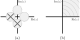
\includegraphics[draft=false, width=0.8\linewidth]{qds/elimsig2}
\caption{\label{fig:qds_elimsig2} Multiple heterodyne outcomes give rise to the same eliminated signature element. (a) A particular eliminated signature element. (b) All possible heterodyne outcomes consistent with (a).}
\end{figure}


Let us use the notation for eliminated signature elements from Tab.~\MT{X}. Consider the first eliminated signature element $e_1$. We mix $\rho_{B | c}$ over all outcomes $c$ which are consistent with $e_1$

\begin{equation}\label{eqn:qds_aposterioristate}
\rho_{B | e_1} = \mathcal{N}\left(e_1\right) \int\limits_{\text{Re}\left(c\right) > 0, \; \text{Im}\left(c\right)>0} \Diff2 c \; \text{P}\left(c\right) \; \rho_{B | c},
\end{equation}
with the normalization factor defined as\footnote{Clearly the $\mathcal{N}$ as defined in Eq.~\ref{eqn:qds_aposterioristate_normalization} is equal to $1/4$ for each $e_1, e_2, e_3, e_4$. We show Eq.~\ref{eqn:qds_aposterioristate_normalization} here for completeness, though it will become important in Sec.~\ref{sec:qds_postselection} when we discuss postselection on measurement outcomes, and in Ch.~\ref{chapter:aqc} when assumptions about uniform sending probabilities are relaxed.}
\begin{equation}\label{eqn:qds_aposterioristate_normalization}
\frac{1}{\mathcal{N}\left(e_1\right)} = \int\limits_{\text{Re}\left(c\right) > 0, \; \text{Im}\left(c\right)>0} \Diff2 c \; \text{P}\left(c\right).
\end{equation}

\noindent The conditional state $\rho_{B|e_1}$ is the quantum state held by Bob when Charlie has received eliminated signature element $e_1$. Bob's states conditioned on eliminated signature elements $e_2, e_3, e_4$ are calculated likewise by varying the limits of integration.

Bob's \emph{a posteriori} entropy Eq.~\ref{eqn:intro_aposteriori} thus reads
\begin{equation}
S_{\text{aposteriori}} = \sum_{e_k} \text{P}\left(e_k\right) S\left(\rho_{B | e_k}\right)
\end{equation}
in terms of Von Neumann entropy $S$. In this chapter we are working in the ideal case where each eliminated signature element is equally likely, and where the entropies of each of the $\rho_{B | e_k}$ are equal, and so we simply write Bob's \emph{a posteriori} entropy as

\begin{equation}\label{eqn:aposteriori_entropy}
S_{\text{aposteriori}} = S\left(\rho_{B | e_1}\right).
\end{equation}

\noindent Bob's \emph{a priori} state is given by
\begin{equation}\label{eqn:qds_aprioristate}
\rho_{\text{apriori}} = \sum_{e_k} \text{P}\left(e_k\right) \rho_{B|e_k}
\end{equation}
with corresponding \emph{a priori} entropy Eq.~\ref{eqn:intro_apriori} simply $S\left(\rho_{\text{apriori}}\right)$, and where $\text{P}\left(e_k\right)$ is here equal to $1/4$. %Note that the state Eq.~\ref{eqn:qds_aprioristate} is equivalent to the \emph{a posteriori} state Eq.~\ref{eqn:qds_aposterioristate} when the integration limit is extended over the entire complex plane. 
Finally, using the definiition of Holevo information, Eq.~\ref{eqn:intro_holevo}
\begin{equation}
\chi = S_{\text{apriori}} - S_{\text{aposteriori}}.
\end{equation}
we calculate and plot $\chi$ under attack $BS0$ in Fig.~\ref{fig:qds_holevo_comparisons}. 

\subsubsection{$BS1$: $\xi > 0$}\label{sec:qds_bs1}
\begin{figure}[htp]
\centering
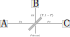
\includegraphics[draft=False, width=0.8\linewidth]{qds/BS1}
\caption{\label{fig:bs1_attack} Attack BS$1$. The beamsplitter mimics channel loss, while the mixing with thermal state $\rho_{\text{thermal}}$ introduces excess noise into Charlie's outcome.}
\end{figure}
Next let us consider a modification to canonical attack $BS0$ which will allow for modelling of channels which induce excess noise at Charlie. In this attack, denoted $BS1$ and displayed in Fig.~\ref{fig:bs1_attack}, Eve inputs a thermal state Eq.~\MT{X} into the fourth port of the beamsplitter. Let us analyse its effect on Holevo information. Its effect on Charlie's measurement outcomes is discussed above in Sec.~\MT{X} \MT{Make sure I do this}.

We wish to mix a coherent state $\rho_{\alpha_k} = \dyad{\alpha_k}$ and a thermal state $\rho_{\text{thermal}}$ on a beamsplitter with transmittivity $T$. In Fock basis our states take the following form

\begin{align}
&\rho_{\alpha_k} = e^{-\left|\alpha_k\right|^2} \sum_{n, m=0}^{\infty} \frac{\alpha_k^n \overline{\alpha_k}^{m}}{\sqrt{n! m!}} \dyad{n}{m} \notag \\
&\rho_{\text{thermal}} = \left(1 - e^{-\tilde{\beta}}\right) \sum_{p=0}^\infty e^{- p \tilde{\beta}}\dyad{p} \qq{with} \tilde{\beta} = \log_e\left(\frac{1}{\bar{n}} +1\right)
\end{align}

\noindent and so the input state into the beamsplitter is
\begin{equation}
\rho_{\text{input}} = \rho_{\alpha_k} \otimes \rho_{\text{thermal}}.
\end{equation}

\noindent Enacting beamsplitter relation Eq.~\MT{X} on $\rho_{\text{input}}$, we arrive at our two-mode output state shared between Bob and Charlie.
%\begin{align}
%%
%&\rho_{\text{output}} = \sum_{n, m, p=0}^\infty e^{- \left| \alpha_k \right|^2}\left(1 - e^{- \tilde{\beta}}\right) \frac{\alpha_k^n \overline{\alpha_k}^m}{\sqrt{n! m!}} e^{- p \tilde{\beta}} \sqrt{n! p! m! p!} \notag \\
%%
%&\sum_{k_1, k_2, l_1, l_2=0}^{n, p, m, p} \pmqty{n \\ k_1} \pmqty{p \\ k_2} \pmqty{m \\ l_1} \pmqty{p \\ l_2} \left(\sqrt{T}\right)^{k_1 + l_1} \left(\sqrt{1-T}\right)^{n + m - k_1 - l_1} \notag \\
%%
%&\left(-\sqrt{1-T}\right)^{k_2 + l_2} \left(\sqrt{T}\right)^{2 p - k_2 - l_2} \sqrt{\left(k_1 + k_2\right)! \left(n + p - k_1 - k_2\right)!} \notag \\
%%
%&\sqrt{\left(l_1 + l_2\right)! \left(m + p - l_1 - l_2\right)!}
%%
%\dyad{k_1 + k_2, n + p - k_1 - k_1}{l_1 + l_2, m + p - l_1 - l_2}
%\end{align}
%\MT{make equation prettier. And decide whether I even want to include it.}
Heterodyning on Charlie's mode using POVM Eq.~\MT{X}, we see that Bob's sub-normalized conditional state is

\MT{I think I should display Bob's sub-normalized conditional state, since I will then obviously work with it, but perhaps it is a waste of space to display the two-mode state? I can speak to NK about it}

\begin{align}\label{eqn:qds_bs1_deriv_2}
%
&\tilde{\rho}_B\left(c\right) = \frac{e^{-\left|\alpha_k\right|^2}}{\pi}\left(1 - e^{-\tilde{\beta}}\right) \sum_{n, m, p=0}^\infty \frac{\alpha_k^n \overline{\alpha_k}^m}{\sqrt{n! m!}} e^{- p \tilde{\beta}} \sqrt{n! p! m! p!} \notag \\
%
&\sum_{k_1, k_2, l_1, l_2=0}^{n, p, m, p} \pmqty{n \\ k_1} \pmqty{p \\ k-2} \pmqty{m \\ l_1} \pmqty{p \\ l_2} \left(\sqrt{T}\right)^{k_1 + l_1} \left(\sqrt{1-T}\right)^{n + m - k_1 - l_1} \notag \\
%
&\left(-\sqrt{1-T}\right)^{k_2 + l_2} \left(\sqrt{T}\right)^{2 p - k_2 - l_2} \sqrt{\left(n + p - k_1 - k_2\right)!} \notag \\
%
&\sqrt{\left(m + p - l_1 - l_2\right)!} \dyad{n + p - k_1 - k_2}{m + p - l_1 - l_2} \delta_{k_1+k_2}^{l_1+l_2} \left[ e^{-\left|c\right|^2} c^{k_1 + k_2} \overline{c}^{l_1 + l_2} \right]
%
\end{align}
\MT{make this equation pretty. Also introduce somewhere the tilde notation to convey a sub-normalized state}
where $\delta_k^l$ is the Kronecker delta which arises after tracing out Charlie's mode.

\MT{I've gotta remember to mix it over $\alpha_k$.} Now, to reach the \emph{a posteriori} state under this attack we will integrate this $\tilde{\rho}_B$, as in Eq.~\ref{eqn:qds_aposterioristate}. This will correspond to simply integrating the scalar terms involving $c$, noting that the integration operation will commute with the rest of state Eq.~\ref{eqn:qds_bs1_deriv_2}. Note also that we may neglect the $\text{P}\left(c\right)$ term from the integrand Eq.~\ref{eqn:qds_aposterioristate}, since our state is already sub-normalized by precisely the required factor. 

The integration is best performed in Polar coordinates since radial and azimuthal integrands separate. So we find
\begin{align}\label{eqn:qds_bs1_deriv_3}
\int\limits_{\text{Re}\left(c\right)>0, \text{Im}\left(c\right)>0} \Diff2 c \; &e^{-\left|c\right|^2} c^k \overline{c}^l = \notag \\
&\begin{cases}
\frac{\pi}{4} \Gamma\left(k+1\right) & \text{if } k = l \\
\frac{-i}{k-l}\left(-1 + e^{i \frac{\pi}{2}\left(k-l\right)}\right)\frac{1}{2}\Gamma\left(\frac{1}{2}\left(k + l + 2\right) \right) & \text{if } k \ne l
\end{cases}
\end{align}
with $\Gamma$ the gamma function. Indeed, the radial component of the integrand of Eq.~\ref{eqn:qds_bs1_deriv_3} is a standard integral for $\Gamma$. The final \emph{a posteriori} state is now accessible. \MT{still gotta calculate the normalization factor}

The \emph{a posteriori} state is calculated likewise, but the limits of integration should be extended to the entire complex plane. In this case,
\begin{equation}\label{eqn:qds_bs1_deriv_4}
\int\limits_{\mathbb{C}} \Diff2 c \; e^{-\left|c\right|^2}c^k \overline{c}^l = \pi \Gamma\left(k+1\right)
\end{equation}
since the polar integral forces $k=l$.


\MT{Now let us talk about how $\text{P}\left(c\right)$ is affected by noise. (first, I should understand how the heterodyne povm is derived and where factors of sqrt2 should appear)}


\MT{summary paragraph:}
The Holevo information may now be calculated in the usual way, and we compare Holevo information under different attacks in Fig.~\ref{fig:qds_holevo_comparisons}.
\MT{where do I want to talk about truncating matrices and numerical methods?}

\subsubsection{$BS2$: $\xi > 0$}\label{sec:qds_bs2}
We now introduce and consider a second modification to the usual beamsplitter attack, which will allow the excess noise on the channel to be modelled. This attack can be viewed as an unphysical combination of the previous two attacks which advantages Bob and disadvantages honest parties.

As we see in Fig.~\ref{fig:qds_holevo_comparisons}, below, Bob performs worse under $BS1$ than $BS0$. This is a consequence of the fact that the input noise also affects his own measurements and so will reduce his information about Charlie's output. So we modify the beamsplitter attack by imposing that the channel excess noise should only affect honest players. That is, the presence of $\xi$ causes $\perr$ to increase, but Holevo information and therefore $\pe$ should both be unaffected. 

While strictly this attack is physically inconsistent, and therefore unphysical, it is more pessimistic than either $BS0$ or $BS1$, and so the security bounds it gives are preferable to either of those attacks. The Holevo information is given by using Eqs.~\ref{eqn:qds_aposterioristate} and \ref{eqn:qds_aprioristate} in the usual way, while $\perr$ is given by Eq.~\ref{fig:qds_holevo_comparisons}. The performance of this attack is analysed in Fig.~\MT{X}.

\subsection{Entangling-cloner attack}
\begin{figure}[htp]
\centering
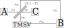
\includegraphics[draft=False, width=0.8\linewidth]{qds/EC}
\caption{\label{fig:ec_attack} EC attack. Locally, one mode of the TMSV looks like $\rho_{\text{thermal}}$, and so allows channel excess noise to be emulated. Bob can exploit correlations in noise between his two mode output state $\rho_{B_1^\prime, B_2}$ to gain additional information.}
\end{figure}
The entangling cloner attack, depicted in Fig.~\ref{fig:ec_attack}, is ideally suited to consistently incorporate the presence of excess noise $\xi$, and we shall see that it is a much more powerful attack than any of the beamsplitter attacks considered above. The entangling cloner attack, which we shall denote $EC$, may be viewed as a natural extension of attack $BS1$, above. Instead of inputting a thermal state into the beamsplitter's fourth port, Bob will input one arm of his entangled two-mode squeezed vacuum (TMSV) state. The mode which Bob inputs into the channel is locally indistinguishable from $\rho_{\text{thermal}}$, and so honest players cannot tell which of these attacks is being performed. 

The $EC$ attack has a long history, and is known to be the optimal collective attack for gPSK QKD \MT{cite a bunch of stuff}. Since our QPSK alphabet is non-Gaussian we make no claims as to $EC$'s optimality, though we conjecture that $EC$ will be optimal as $\alpha \rightarrow 0$, and close to optimal for $\alpha << 1$. The status of optimal attacks on QDS is an open one and should be the subject of further exploration. The question about optimal attacks on QKD with discrete modulated coherent states is also open, despite a long history of activity on these protocols. In any case, the $EC$ attack is very difficult to perform with today's technology, and so a protocol with security against $EC$ (or even $BSx$) attacks should be expected to be practically secure for a long time.

\MT{Talk somewhere about where the extra power in the EC attack comes from - we allow Bob to exploit also the correlations between his two modes. Also have some figures of histograms of this attack}

Let us analyse the $EC$ attack. Alice creates the coherent state $\rho_{\alpha_k}$ (Eq.~\MT{X}), while Bob creates
\begin{equation}
\tmsv = \frac{1}{\cosh^2 \zeta}  \sum_{n, m=0}^\infty \left(\tanh\zeta\right)^{n+m} \dyad{n, n}{m, m}.
\end{equation}

\noindent Let us write the three-mode input state to the channel as

\begin{align}
\rho_{\text{input}} &= \frac{e^{-\left|\alpha_k\right|^2}}{\cosh^2 \zeta} \sum_{n_1, m_1=0}^\infty \sum_{n_2, m_2=0}^{\infty} \frac{\alpha_k^{n_1} \overline{\alpha_k}^{m_1}}{\sqrt{n_1! m_1!}} \left(\tanh\zeta\right)^{n_2 + m_2} \notag \\
&\times \bigg[\dyad{n_1, n_2}{m_1, m_2}\bigg] \otimes \dyad{n_2}{m_2}
\end{align}

\noindent where we have explicitly separated in square brackets the two modes which will interfere on the beamsplitter.

The beamsplitter mixes $\dyad{n_1, n_2}{m_1, m_2}$ via Eq.~\MT{X}, and gives an entangled three-mode state at the output. Charlie heterodynes on his mode and receives outcome $c$, and we arrive at Bob's sub-normalized two-mode output state:

\begin{align}\label{eqn:qds_ec_deriv_1}
&\tilde{\rho}_{B}\left(c\right) =  \frac{e^{-\left|\alpha_k\right|^2}}{\cosh^2\zeta} \frac{1}{\pi} \sum_{n_1, m_1, n_2, m_2 = 0}^\infty \alpha_k^{n_1} \overline{\alpha_k}^{m_1} \left(\tanh\zeta\right)^{n_2 + m_2} \sum_{k_1, k_2, l_1, l_2 = 0}^{n_1, n_2, m_1, m_2}  \notag \\
%
&\sqrt{n_2! m_2!} \left(\sqrt{T}\right)^{k_1 + l_1} \left(\sqrt{1-T}\right)^{n_1 + m_1 - k_1 - l_1} \left(-\sqrt{1-T}\right)^{k_2 + l_2} \left(\sqrt{T}\right)^{n_2 + m_2 - k_2 - l_2} \notag \\
%
&\times \sqrt{\left(n_1 + n_2 - k_1 - k_2\right)! \left(m_1 + m_2 - l_1 - l_2\right)} \notag \\
%
&\times \left[k_1! k_2! l_1! l_2! \left(n_1 - k_1\right)! \left(n_2 - k_2\right)! \left(m_1 - l_1\right)! \left(m_2 - l_2\right)! \right]^{-1} \notag \\
%
&\times \dyad{n_1 + n_2 - k_1 - k_2}{m-1 + m_2 - l_1 - l_2} \otimes \dyad{n_2}{m_2} \notag \\
%
&\times \left[e^{-\left|c\right|^2} c^{k_1 + k_2} \overline{c}^{l_1 + l_2} \right]
\end{align}

\noindent where we have again separated the terms involving $c$. Once again the state is readily integrated in $c$, either over the entire complex plane or a single quadrant, and we may simply substitute Eqs.~\ref{eqn:qds_bs1_deriv_3},~\ref{eqn:qds_bs1_deriv_4} into Eq.~\ref{eqn:qds_ec_deriv_1} to reach the \emph{a posteriori} and \emph{a priori} states, respectively.

The \emph{a priori} state is automatically normalized by virtue of the integration over $\mathbb{C}$, while the \emph{a posteriori} state is normalized by multiplying by $\mathcal{N}\left(e_1 \given \xi \right)$, defined as 

\begin{equation}
\frac{1}{\mathcal{N}\left(e_1 \given \xi\right)} = \int\limits_{\text{Re}\left(c\right) > 0, \; \text{Im}\left(c\right)>0} \Diff2 c \; \text{P}\left(c \given \xi \right).
\end{equation}
where we have included excess noise $\xi$ in our probability, as in Eq.~\MT{X}.




\begin{figure}
\includegraphics{qds_holevo_comparisons.png}
\caption{\label{fig:qds_holevo_comparisons}}
\end{figure}


\section{Signature length $L$}
\MT{better segue}
We now wish to calculate the total probability $\varepsilon_{\text{fail}}$ that our QDS protocol fails by any of the routes discussed earlier: by allowing Alice to repudiate, by allowing Bob to forge, or by aborting even in the absence of attack.

For a figure of merit, we will assume that the protocol will fail in any of these ways with equal probability, and so we set
\begin{equation}
\varepsilon_{\text{fail}} = \varepsilon_{\text{honest abort}} = \varepsilon_{\text{repudiation}} = \varepsilon_{\text{forgery}},
\end{equation}
though we note that alternative combinations could be considered. Let us eliminate free parameters $s_B, s_C$ by equating the arguments of Eqs.~\ref{eqn:erep},~\ref{eqn:ehonabort},~\ref{eqn:eforg}
\begin{equation}
\left(\pe - s_C\right)^2  = \frac{1}{4}\left(s_C - s_B\right)^2 = \left(s_B - \perr\right)^2
\end{equation}
from which we may derive
\begin{equation}
s_B = \frac{3}{4} \perr + \frac{1}{4}\pe \qq{and} s_C = \frac{1}{4}\perr + \frac{3}{4}\pe
\end{equation}
as our choices of security thresholds. Notice that since $\perr \le \pe$ we automatically fulfil $s_B \le s_C$. The overall probability of failure becomes

\begin{equation}\label{eqn:efail}
\varepsilon_{\text{fail}} \le 2 \text{exp}\left( - \left[\pe - \perr\right]^2 \frac{L}{16}\right).
\end{equation}




\section{Postselection}
In the context of QKD it has been known for some time that postselection of measurement outcomes will improve the key rates in the presence of excess noise, and is even a requirement to distill a key below $T \le 1/2$ in the direct reconciliation regime \MT{cite some stuff}. We are thus motivated to apply postselection to our QDS protocol in order to allow a message to be securely signed over a larger range of channel parameters. The results of this section will be useful in Ch.~\MT{X} where--as for DR QKD--we shall see that postselection is a necessity for some QDS protocols.

To apply the postselection technique, recipients Bob and Charlie in the protocol will simply disregard unfavourable measurement outcomes, i.e. outcomes for which a dishonest player is deemed to have too much knowledge, or for which the probability of honest mismatch is too high.

We thus define a region $\rps \in \mathbb{C}$, Fig.~\ref{fig:rps}. Honest recipients will only accept measurement outcomes $x \in \mathbb{C}\setminus\rps$. We will vary $\rps$ in order to increase the range of channel parameters for which the QDS protocol is secure, and to minimize signature length $L$.

\begin{figure}[htp]
\centering
\includegraphics[draft=false, width=0.5\linewidth]{qds/rps}
\caption{\label{fig:rps} The postselection region $\rps$, gray, is parametrized by $\Delta_r, \Delta_\theta$ in polar coordinates. Participants will only accept measurement outcomes $x \in \mathbb{C} \setminus \rps$. }
\end{figure}

To be concrete, we allow $\rps$ to be parametrized by two variables $\Delta_r, \Delta_\theta$ in polar coordinates, Fig.~\ref{fig:rps}. This is the same postselection region which was considered in the recent work \MT{cite}, but if desired more general regions may be readily considered. We make no claims as to the optimality of our choice of the shape $\rps$, though once the form of $\rps$ is set, $\Delta_r$ and $\Delta_\theta$ may be readily optimized over.

The crucial quantity which controls the security of our QDS protocol is $g_{\text{sec}} = \pe - \perr$, which describes the performance advantage which an honest player has over a dishonest player. The protocol is secure provided that $g_{\text{sec}} > 0$. We therefore must consider how postselection affects $g_{\text{sec}}$. 

Let us begin with the effect of postselection on $\perr = \perr\left(\Delta_r, \Delta_\theta\right)$. \MT{I don't want to talk yet about calculating $\perr$ from data - that should wait until the agile chapter.} Recall that when Alice sends state $\ket{\alpha}$ through a lossy channel, transmittivity $T$, Charlie receives outcome $x \in \mathbb{C}$ with probability

\begin{equation}
\text{P}\left(x \given \alpha, T\right) = \frac{1}{\pi} \exp\left( - \left| x - \sqrt{\frac{T}{2}}\alpha\right|^2\right).
\end{equation}

\noindent Thus the probability of eliminating the state $\ket{\alpha}$ when no postselection is used is, in polar coordinates,
\begin{align}
\perr &= \int\limits_{r=0}^\infty \mathrm{d}r \; r \int\limits_{\theta = \pi/2}^{3 \pi/2} \mathrm{d}\theta \; \text{P}\left(r e^{i \theta} \given \alpha, T\right) \notag \\
%
&= \frac{1}{2}\erfc\left(\sqrt{\frac{T}{2}}\left|\alpha\right|\right).
\end{align}

\noindent Ignoring region $\rps$ from our integral, the mismatch probability becomes

\begin{align}\label{eqn:perrps_deriv_2}
\perr\left(\Delta_r, \Delta_\theta\right) = \frac{1}{\mathcal{N}} \int\limits_{\Delta_r}^{\infty} \mathrm{d}r \; r &\left[ \; \int\limits_{ \pi/2 + \Delta_\theta}^{\pi - \Delta_\theta} \mathrm{d}\theta \; \text{P}\left(r e^{i \theta} \given \alpha, T\right) \right. \notag \\
%
&\left. \int\limits_{3 \pi/2 - \Delta_\theta}^{\pi + \Delta_\theta} \mathrm{d}\theta \; \text{P}\left(r e^{i \theta} \given \alpha, T\right) \right],
\end{align}

\noindent where normalization probability $\mathcal{N}$ is the probability that Charlie will accept his measurement outcome, which is calculated by extending the integration in Eq.~\ref{eqn:perrps_deriv_2} to the entire $\mathbb{C} \setminus \rps$.

The calculation of $\perrps$ follows identically when excess noise $\xi$ is included, simply using the requisite formulae Eqs.~\MT{X} and performing the integrations as above. 

\MT{Remember to talk later about how $L$ should be rescaled.}

Since a dishonest player's declaration will depend on an honest player's heterodyne outcome, the probability $\pe$ must also vary with $\rps$. We will calculate the effect of $\rps$ on Holevo information $\chi$. Probability $\pe$ is then calculated via Eq.~\ref{eqn:qds_hpe} as normal.

Let Bob's $j^{\text{th}}$ \emph{a posteriori} state be $\rho_{B | e_k}^j$, which is conditioned on Charlie holding eliminated signature element $e_k$, and $1\le j \le L/2$. Assume that Bob has performed any one of the attacks examined in Sec.~\ref{sec:attack_analysis}, and let Bob's state after Charlie's heterodyne measurement be denoted $\rho_{B | c}^j$. Again, since Charlie's eliminated signature element is entirely determined by the quadrant in which $c$ lies, the state $\rho_{B | e_k}^j$ is calculated by mixing $\rho_{B | c}^j$ over an entire quadrant of phase-space, as in Eqs.~\ref{eqn:qds_aposterioristate},~\ref{eqn:qds_bs1_deriv_3}. We must therefore update these integrals to include the effect of $\rps$. For example,

\begin{align}\label{eqn:qdsps_aposteriori}
\tilde{\rho}_{B | e_1}^j &= \frac{1}{\mathcal{N}} \int \Diff2 c \; \rho_{B | c}^j \notag \\
%
&=\frac{1}{\mathcal{N}} \int\limits_{\Delta_r}^\infty \mathrm{d}r\; r\int\limits_{\Delta_\theta}^{\pi/2 - \Delta_\theta} \mathrm{d}\theta \; \rho_{B | r e^{i \theta}},
\end{align}

\noindent and similarly for $e_2, e_3, e_4$ with updated limits of the $\theta$ integral. The $\mathcal{N}$ is identical to that from Eq.~\ref{eqn:perrps_deriv_2}. The $\emph{a priori}$ state is likewise found by mixing Eq.~\ref{eqn:qdsps_aposteriori} over all quadrants, and thus $\pe\left(\Delta_r, \Delta_\theta\right)$ may be calculated via Eq.~\ref{eqn:qds_hpe}. \MT{gotta talk about how we actually perform the integration}

We may again separate out terms involving $c$, and so the integration from Eq.~\ref{eqn:qdsps_aposteriori} becomes

\begin{equation}
\frac{1}{\mathcal{N}} \int\limits_{\Delta_r}^{\infty} \mathrm{d}r \; r \int\limits_{\Delta_\theta}^{\pi/2 - \Delta_\theta} \mathrm{d}\theta \; r^k r^l e^{-r^2} e^{i \theta \left(k - l\right)}.
\end{equation}

\noindent To perform the integration, it is helpful to perform the angular integral first, which readily integrates to a sum of exponentials when $k \ne l$, or to $\pi/2 - 2\Delta_\theta$ when $k=l$. The remaining radial term is

\begin{equation}
\int\limits_{\Delta_r}^\infty \mathrm{d}r \; r^{k + l + 1} e^{-r^2}
\end{equation}

\noindent which is the definition of an upper incomplete Gamma function \MT{cite mathworld}, which we denote as $\Gamma_\uparrow$. The radial integration is thus identically

\begin{equation}
\Gamma_{\uparrow}\left(\frac{1}{2}\left[2 + k + l\right], \Delta_r^2\right)  \forall k, l \ge 0
\end{equation}
which may be easily calculated.

We have now included the effects of $\rps$ on $g_{\text{sec}}$, and so the performance of the protocol under postselection may be analysed.

\MT{Have some graphs showing effect of postselection on $g_{sec}$ under different attacks.}

Let us turn now to examine our main figure of merit, the number of quantum states $L$ used in the protocol. Howver, directly incorporating $g_{\text{sec}}\left(\Delta_r, \Delta_\theta\right)$ into Eq.~\ref{eqn:efail} will give an erroneous level of security, for the following reason. Our calculations in this section, culminating in $g_{\text{sec}}$ may be used to bound the number of states required to sign a message. However, this is not equivalent to the number of states which Alice has sent. 

For example, choosing $\Delta_r = $\MT{X} and $\Delta_\theta = $\MT{X} gives $g_{\text{sec}} = $\MT{X}. Substituting this into Eq.~\ref{eqn:efail} and solving for $L$ gives $L = $\MT{X} under attack \MT{X}. But in order to have that many states accepted at Charlie, Alice will need to send $\MT{X}$ coherent states in total, since Charlie will reject his measurement outcomes with probability \MT{X}. It follows that $L$, as implicitly defined in Eq.~\ref{eqn:efail} is a poor figure of merit to measure the resource-use of our protocol when postselection is used.

Instead, we will work in terms of $\tilde{L}$, which we define as the total number of states sent by Alice. This is a rescaling of $L$ given by
\begin{equation}
L \mapsto \tilde{L} := \frac{L}{\mathcal{N}},
\end{equation}
with $\mathcal{N}$ defined as the average probability that Charlie accepts a given state sent by Alice (see the discussion surrounding Eq.~\ref{eqn:perrps_deriv_2}. 

We plot $\mathcal{N}$ in Fig.~\ref{fig:psnorm}, and figure of merit $\tilde{L}$ is plotted in Fig.~\ref{fig:psl}. \MT{add a discussion of how postselection affects $\tilde{L}$.} 

\begin{figure}[htp]
\centering
\begin{subfigure}{0.4\linewidth}
\includegraphics[draft=false, width=\linewidth]{qds/psnorm1}
\caption{}
\end{subfigure}
\begin{subfigure}{0.4\linewidth}
\includegraphics[draft=false, width=\linewidth]{qds/psnorm2}
\caption{}
\end{subfigure}
\caption{\label{fig:psnorm}}
\end{figure}

\begin{figure}[htp]
\centering
\includegraphics{psl.png}
\caption{\label{fig:psl} Normalization factor $\mathcal{N}$ varies dramatically with postselection region $\rps$. (a) $\alpha=0.5, T=0.5$. (b) $\alpha=3.0, T=1.0$}
\end{figure}



\MT{have a section where I make some remarks about the postselection technique. Note that I have implicitly assumed that Bob knows whether an individual state has been postselected on. This is a sensible assumption for QKD, since it will be declared, but for QDS it does not need to be declared, so I am giving Bob too much power here.}


\section{Protocol performance}
\MT{Let's look at some results and graphs of the protocol performance under the four above attacks. TODO: make graphs like in the PRA paper}


\section{Outlook}


